%%%%%%%%%%%%%%%%%%%%%%%%%%%%%%%%%%%%%%%%%%%%%%%%%%%%%%%%%%%%
\section{General Argument}\label{sec:argument}
%%%%%%%%%%%%%%%%%%%%%%%%%%%%%%%%%%%%%%%%%%%%%%%%%%%%%%%%%%%%

\subsection{Primitive Information and the Rectangle}\label{sec:argument:primitives}

Suppose a researcher observes data generated from a nonparametric regression function $m(x,z) = \E[Y \mid X = x, Z = z]$ and wishes to estimate it nonparametrically.
To conduct minimax optimal inference, the researcher must choose a smoothness class --- a convex set of functions over which worst-case risk will be evaluated.
A natural first step is to reason about bounds on the partial derivatives:
\begin{equation*}
	\abs*{\frac{\partial m}{\partial x}} \leq M_x, \qquad \abs*{\frac{\partial m}{\partial z}} \leq M_z.
\end{equation*}
These bounds are the researcher's \emph{primitive information}: substantive reasoning about the maximal rate of change in each direction.
The task is to translate these bounds into a smoothness class $\mathcal{F}$ by choosing a \emph{gradient constraint set} $\mathcal{C} \subset \mathbb{R}^2$ --- a set of feasible gradient pairs $(\partial m / \partial x,\, \partial m / \partial z)$ --- and defining $\mathcal{F}(\mathcal{C}) = \{ f : \nabla f(x,z) \in \mathcal{C} \text{ for all } (x,z) \}$.

The only structural requirement on $\mathcal{C}$ is convexity: if $f, g \in \mathcal{F}(\mathcal{C})$, then $\nabla(\lambda f + (1-\lambda)g) = \lambda \nabla f + (1-\lambda) \nabla g$ must lie in $\mathcal{C}$.
Convexity of $\mathcal{C}$ is necessary and sufficient for the function class to be closed under convex combinations --- the minimal assumption for a coherent smoothness class and for the minimax machinery that relies on convexity of $\mathcal{F}$.

Another structural restriction, standard in the minimax literature, is centrosymmetry. 

\begin{definition}[Centrosymmetry]\label{def:centrosymmetric}
	A set $\mathcal{C} \subset \mathbb{R}^d$ is \emph{centrosymmetric} if $\mathcal{C} = -\mathcal{C}$, i.e., $u \in \mathcal{C}$ implies $-u \in \mathcal{C}$.
	A function class $\mathcal{F}$ is centrosymmetric if $f \in \mathcal{F}$ implies $-f \in \mathcal{F}$.
	If $\mathcal{C}$ is centrosymmetric, then $\mathcal{F}(\mathcal{C})$ is centrosymmetric.
\end{definition}

Throughout the paper I restrict attention to constraint sets that are nonempty, convex, compact and centrosymmetric, unless stated otherwise.

\begin{definition}[Separable constraint set]\label{def:separable}
	A constraint set $\mathcal{C} \subset \mathbb{R}^2$ is \emph{separable} if it is a Cartesian product of symmetric intervals: $\mathcal{C} = [-A, A] \times [-B, B]$ for some $A, B > 0$.
	In a separable set, each partial derivative is constrained independently --- the feasible range of one does not depend on the value of the other.
\end{definition}

The natural separable class matching the primitive bounds is the rectangle
\begin{equation*}
	\mathcal{C}_s \defeq [-M_x, M_x] \times [-M_z, M_z].
\end{equation*}
It admits every gradient pair individually consistent with the primitives, without imposing any relationship between $\partial m / \partial x$ and $\partial m / \partial z$ and induces the function class $\mathcal{F}(\mathcal{C}_s)$.
\footnote{The separable class has a structural parallel in copula theory. The Fréchet class $\mathcal{F}(F_1, F_2)$ of all joint distributions with marginals $F_1, F_2$ is bounded by the Fréchet--Hoeffding bounds, and the independence copula $C(u,v) = uv$ is the unique element imposing no dependence. The rectangle is to gradient constraint sets what the independence copula is to joint distributions: the Cartesian product of the marginal objects, imposing no cross-coordinate structure \parencite[cf.][Chapter~2]{nelsen_introduction_2006}.} If $M_x \neq M_z$ the separable class contains directional information and is in that sense \textit{anisotropic}. It then resembles anisotropic function classes occasionally used in the minimax literature $\mathcal{F}_1^{\mathrm{aniso}}(M_x, M_z) \defeq \mathcal{F}(\mathcal{C}_s)$.

The separable class encodes the primitive information and nothing more: each partial derivative is constrained independently, with no restriction on how they combine.
But could there be other constraint sets that also respect the primitive information --- that is, sets which do not exclude any individually-permitted gradient pair?

\begin{definition}[Primitive-consistent constraint set]\label{def:primitive_consistent}
	Let $M_x, M_z > 0$.
	A set $\mathcal{C} \subset \mathbb{R}^2$ is \emph{primitive-consistent} with bounds $(M_x, M_z)$ if $\mathcal{C}$ satisfies $\mathcal{C}_s \subseteq \mathcal{C}$: every gradient pair individually permitted by the primitive bounds is also permitted by $\mathcal{C}$.
\end{definition}

Primitive consistency requires that the constraint set does not discard any gradient pair that the researcher's marginal bounds allow.
A class that fails this condition forbids some individually-permitted gradient combination --- it imports information beyond the primitives.

\begin{proposition}[The separable class is the smallest primitive-consistent class]\label{prop:coupling_agnostic}
	For any $M_x, M_z > 0$, the separable class $\mathcal{C}_s = [-M_x, M_x] \times [-M_z, M_z]$ is the smallest primitive-consistent constraint set: any primitive-consistent $\mathcal{C}$ satisfies $\mathcal{C}_s \subseteq \mathcal{C}$.
	The induced function class $\mathcal{F}(\mathcal{C}_s) = \mathcal{F}_1^{\mathrm{aniso}}(M_x, M_z)$ is therefore the smallest function class the researcher can justify from the primitive bounds alone.
\end{proposition}

\begin{proof}
	$\mathcal{C}_s$ is primitive-consistent: $\mathcal{C}_s \subseteq \mathcal{C}_s$.
	Any primitive-consistent $\mathcal{C}$ satisfies $\mathcal{C}_s \subseteq \mathcal{C}$ by definition.
	Hence $\mathcal{C}_s$ is contained in every primitive-consistent set.
	Since $\mathcal{F}(\mathcal{C}_1) \subseteq \mathcal{F}(\mathcal{C}_2)$ whenever $\mathcal{C}_1 \subseteq \mathcal{C}_2$, the induced class $\mathcal{F}(\mathcal{C}_s)$ is the smallest among all primitive-consistent classes.
\end{proof}

The separable class is the tightest encoding of primitive information.
Any primitive-consistent superset admits gradients beyond the marginal bounds, inflating the effective smoothness constants.
Any strict subset forbids individually-permitted gradient pairs, importing information beyond the primitives.
Without additional information about how the partials interact, the researcher cannot justify a class smaller than $\mathcal{C}_s$ --- and any larger primitive-consistent class weakens the resulting inference.


\subsection{Coupling: Non-Separable Constraint Sets}\label{sec:argument:coupling}

\begin{definition}[Coupling]\label{def:coupling}
	A constraint set $\mathcal{C}$ \emph{imposes coupling} if it is not separable --- that is, if it cannot be written as a Cartesian product $[-A, A] \times [-B, B]$ for any $A, B > 0$.
	In a coupled set, the feasible range of one partial derivative depends on the value of the other.
\end{definition}

Coupling amounts to a joint restriction on the primitive bounds --- a budget constraint $h(M_x, M_z) \leq c$ linking the two directions, so that increasing one partial's effective bound requires decreasing the other's.
The leading example is the isotropic disk $B_2(R) = \bigl\{ (u, v) \in \mathbb{R}^2 : u^2 + v^2 \leq R^2 \bigr\}$, which corresponds to the budget constraint $M_x^2 + M_z^2 \leq R^2$: the total gradient budget is $R$, fungible across directions.
A large value of $\partial m / \partial x$ forces a small value of $\partial m / \partial z$, and vice versa.
The isotropic class $\mathcal{F}_1^{\mathrm{iso}}(R) = \mathcal{F}(B_2(R))$ is the standard smoothness class in nonparametric estimation \parencite[e.g.,][]{tsybakov_introduction_2009,stone_optimal_1982}.

Such coupling requires substantive knowledge about the regression function: the researcher must have reason to believe that certain combinations of partial derivatives cannot occur.
In most nonparametric settings --- including density estimation, conditional expectation estimation, and the RDD application of this paper --- such structural beliefs are difficult to justify.
The default, absent strong model-specific reasoning, is to not restrict the partials beyond the primitive bounds.

Non-separable classes face a dichotomy, characterized by whether they contain or exclude the separable class.

\begin{corollary}[Primitive-inconsistent classes add information]\label{cor:coupling_restricts}
	If $\mathcal{C}_s \not\subseteq \mathcal{C}$, then $\mathcal{C}$ is primitive-inconsistent: it excludes individually-permitted gradient pairs, importing information beyond the primitive bounds.
	The induced function class satisfies $\mathcal{F}(\mathcal{C}) \neq \mathcal{F}_1^{\mathrm{aniso}}(M_x, M_z)$.
\end{corollary}

\begin{corollary}[Primitive-consistent supersets inflate bounds]\label{cor:iso_inflates}
	If $\mathcal{C}_s \subsetneq \mathcal{C}$, then $\mathcal{C}$ is primitive-consistent but admits functions with partial derivatives strictly exceeding the primitive bounds: the marginal projections of $\mathcal{C}$ strictly contain $[-M_x, M_x]$ or $[-M_z, M_z]$ (or both).
\end{corollary}

\begin{proof}
	If $\mathcal{C} \supsetneq \mathcal{C}_s$, there exists $(u, v) \in \mathcal{C} \setminus \mathcal{C}_s$, so $\abs{u} > M_x$ or $\abs{v} > M_z$.
	Hence the projection of $\mathcal{C}$ onto the corresponding axis strictly contains the primitive bound.
\end{proof}

\paragraph{The isotropic disk.}
Consider the disk $B_2(R)$ with $R > 0$.
The disk is primitive-inconsistent with bounds $(M_x, M_z)$ whenever $R < \sqrt{M_x^2 + M_z^2}$: the corner $(M_x, M_z)$ of the rectangle satisfies $M_x^2 + M_z^2 > R^2$, so $\mathcal{C}_s \not\subseteq B_2(R)$.
In particular, the inscribed disk with $R \leq \min(M_x, M_z)$ excludes all corners of the rectangle.

Primitive consistency requires $\mathcal{C}_s \subseteq B_2(R)$, which holds if and only if $R \geq \sqrt{M_x^2 + M_z^2}$.
But then the disk inflates the per-partial bounds: the marginal projections of $B_2(R)$ are $[-R, R]$ on each axis, giving inflation factors
\begin{equation*}
	\frac{R}{M_x} = \sqrt{1 + \frac{M_z^2}{M_x^2}} \quad \text{along } x, \qquad \frac{R}{M_z} = \sqrt{1 + \frac{M_x^2}{M_z^2}} \quad \text{along } z.
\end{equation*}
In the symmetric case $M_x = M_z = M$, both factors equal $\sqrt{2}$: the disk inflates each primitive bound by $\sqrt{2}$.

Non-separable classes thus face a dichotomy: they either discard primitive information (\cref{cor:coupling_restricts}) or inflate the primitive bounds (\cref{cor:iso_inflates}).
The separable class $\mathcal{C}_s$ is the unique class that does neither --- the tightest primitive-consistent encoding of the researcher's information.
From an information-theoretic perspective, the rectangle encodes exactly the researcher's primitive information and nothing more: any further restriction is an additional assumption on the relation between the partial derivatives.


\subsection{From Geometry to Minimax Risk}\label{sec:argument:risk}

The geometry of the constraint set $\mathcal{C}$ enters the minimax problem through its \emph{support function}:
\begin{equation*}
	h_{\mathcal{C}}(v) = \sup\bigl\{ \langle u, v \rangle : u \in \mathcal{C} \bigr\}, \qquad v \in \mathbb{R}^2.
\end{equation*}
For the two constraint sets of interest:
\begin{alignat*}{2}
	&\text{Rectangle } [-M_x, M_x] \times [-M_z, M_z]: &\quad h_{\mathrm{rect}}(v) &= M_x \abs{v_1} + M_z \abs{v_2}, \\
	&\text{Disk } B_2(R),\; R = \sqrt{M_x^2 + M_z^2}: &\quad h_{\mathrm{disk}}(v) &= R \norm{v}_2.
\end{alignat*}

The modulus of continuity --- the fundamental quantity governing minimax risk --- depends on $\mathcal{C}$ only through $h_{\mathcal{C}}$ (\cref{cor:modulus_functional} below).
The chain from geometry to risk is:
\begin{enumerate}
	\item $\mathcal{C}_{\mathrm{rect}} \subsetneq \mathcal{C}_{\mathrm{disk}}$ (by \cref{prop:coupling_agnostic} and \cref{cor:iso_inflates}: the disk is primitive-consistent only if $R \geq \sqrt{M_x^2 + M_z^2}$, making it a strict superset of the rectangle).
	\item $\mathcal{F}(\mathcal{C}_{\mathrm{rect}}) \subseteq \mathcal{F}(\mathcal{C}_{\mathrm{disk}})$ (definitional: tighter gradient constraint $\implies$ smaller function class).
	\item $\omega(\delta; \mathcal{F}(\mathcal{C}_{\mathrm{rect}})) \leq \omega(\delta; \mathcal{F}(\mathcal{C}_{\mathrm{disk}}))$ for all $\delta > 0$ (monotonicity of the modulus, \cref{thm:monotonicity}).
	\item $R^*(\mathcal{F}(\mathcal{C}_{\mathrm{rect}})) \leq R^*(\mathcal{F}(\mathcal{C}_{\mathrm{disk}}))$ (minimax risk is governed by the modulus).
\end{enumerate}
The monotonicity proof goes directly through set inclusion --- no support function computation needed.
The support function representation is explanatory: it shows \emph{why} the modulus is monotone (larger $\mathcal{C}$ means pointwise larger $h_{\mathcal{C}}$, which loosens the constraints in the modulus optimization) and will be used to characterize the exact ratio $\rho(M_x, M_z) = R^*(\mathcal{F}(\mathcal{C}_{\mathrm{disk}})) / R^*(\mathcal{F}(\mathcal{C}_{\mathrm{rect}})) > 1$.


\subsection{Application to Optimized RDD}\label{sec:argument:rdd}

Following \textcite{imbens_optimized_2019}, consider a convex weighted average treatment effect:
\begin{equation*}
	\tau_w \defeq \int \tau(c, z)\, w(z)\, dz,
\end{equation*}
where $w(z)$ is a researcher-chosen weight function.
A standard linear RDD estimator uses weights $w_i = w(X_i)$ depending only on the running variable.
A \emph{covariate-adjusted} estimator generalizes to weights $w_i = w(X_i, Z_i)$ that also depend on the covariate $Z_i$, allowing it to exploit the bivariate structure of the design.

Under the isotropic class, covariate adjustment is pointless: the curvature budget is fungible, and the adversary reallocates the entire budget into $x$ (setting $\partial m / \partial z = 0$), rendering $Z$ uninformative.
Under the anisotropic class, the $M_z$ budget cannot be redirected.
Covariate adjustment neutralizes the $z$-channel, stranding the $M_z$ budget; worst-case risk depends primarily on $M_x$, yielding a strict improvement.

The optimal weights, worst-case risk, and confidence intervals in the \textcite{imbens_optimized_2019} framework all depend on $h_{\mathcal{C}}$.
Replacing the isotropic disk with the anisotropic rectangle yields strictly shorter confidence intervals and lower worst-case MSE --- without changing the data, the estimator form, or the target parameter.

\paragraph{Pooling and the tuple function space.}
The comparison of estimators that target different derived quantities of the same DGP requires a common parameter space.
Define four function classes as tuples $(m,\, f_{Z|X},\, \bar{m})$ linked by consistency $\bar{m}(x) = \int m(x,z)\, f_{Z|X}(z \given x)\, dz$:
\begin{align*}
	\mathcal{F}^R(M_x, M_z, L) &\defeq \bigl\{ (m, f_{Z|X}, \bar{m}) : m \in \mathcal{F}_1^{\mathrm{aniso}}(M_x, M_z),\; f_{Z|X} \in \mathcal{F}_1(L),\; \text{consistency} \bigr\}, \\
	\mathcal{F}^{\mathrm{aniso}}(M_x, M_z) &\defeq \bigl\{ (m, f_{Z|X}, \bar{m}) : m \in \mathcal{F}_1^{\mathrm{aniso}}(M_x, M_z) \bigr\}, \\
	\mathcal{F}^{\mathrm{iso}}(R) &\defeq \bigl\{ (m, f_{Z|X}, \bar{m}) : m \in \mathcal{F}_1^{\mathrm{iso}}(R) \bigr\}, \\
	\mathcal{F}^P(M_x^P) &\defeq \bigl\{ (m, f_{Z|X}, \bar{m}) : \bar{m} \in \mathcal{F}_1(M_x^P) \bigr\}.
\end{align*}
By the Leibniz rule, $\abs{\bar{m}'(x)} \leq M_x + M_z \cdot L \eqdef M_x^P$: the pooled Lipschitz constant is derived, not assumed.
The inclusion chain is:
\begin{equation*}
	\mathcal{F}^R \;\subseteq\; \mathcal{F}^{\mathrm{aniso}} \;\subseteq\; \mathcal{F}^{\mathrm{iso}}, \qquad
	\mathcal{F}^R \;\subseteq\; \mathcal{F}^{\mathrm{aniso}} \;\subseteq\; \mathcal{F}^P.
\end{equation*}
The segmented estimator's bias depends only on the $m$-component, so $R^*(\mathcal{F}^R) = R^*(\mathcal{F}^{\mathrm{aniso}})$: the density bound does not bind.
The local constant estimator faces the inflated $M_x^P$, giving:
\begin{equation*}
	R^*(\mathcal{F}^R) \;=\; R^*(\mathcal{F}^{\mathrm{aniso}}) \;\leq\; \min\bigl\{ R^*(\mathcal{F}^{\mathrm{iso}}),\; R^*(\mathcal{F}^P) \bigr\}.
\end{equation*}
\commentT{Coupling and pooling are orthogonal information-loss mechanisms in the tuple space.  Coupling changes the shape of the $m$-cross-section (rectangle $\to$ disk); pooling projects from $(m, f_{Z|X})$ onto $\bar{m}$.  Both inflate the effective Lipschitz constant and increase minimax risk, but through different geometric operations.  Develop into a remark with a schematic figure.}


\subsection{The Prevalence of Isotropic Assumptions}\label{sec:argument:prevalence}

The isotropic class is the default throughout the nonparametric estimation literature --- and in the RDD literature specifically --- despite the coupling it silently imports.
This subsection reviews the key examples and argues that the anisotropic class should be the default whenever the researcher reasons about smoothness from per-direction primitives.

\paragraph{Imbens and Wager (2019).}
The optimized RDD framework of \textcite{imbens_optimized_2019} assumes that the conditional response functions $\mu_w(x) = \E[Y_i(w) \mid X_i = x]$ have bounded second derivatives.
In the univariate case ($X_i \in \mathbb{R}$), the assumption is $\abs{\mu''_w(x)} \leq B$ --- a scalar bound on a scalar quantity, where no iso\-tropic/aniso\-tropic distinction arises.
In the multivariate extension (their Section~II.B), the assumption becomes
\begin{equation*}
	\norm{\nabla^2 \mu_w(x)} \leq B,
\end{equation*}
where $\norm{\cdot}$ is the operator norm (largest absolute eigenvalue of the Hessian).
This is the second-order analog of the isotropic gradient norm constraint $\norm{\nabla f}_2 \leq M$.
It couples the second partial derivatives: large curvature $\partial^2 \mu_w / \partial x^2$ in the running variable direction forces small curvature $\partial^2 \mu_w / \partial z^2$ in the covariate direction.
The total curvature budget $B$ is fungible across directions.

The anisotropic alternative at second order would impose separate bounds:
\begin{equation*}
	\abs*{\frac{\partial^2 \mu_w}{\partial x^2}} \leq B_x, \qquad \abs*{\frac{\partial^2 \mu_w}{\partial z^2}} \leq B_z, \qquad \abs*{\frac{\partial^2 \mu_w}{\partial x \partial z}} \leq B_{xz},
\end{equation*}
constraining the Hessian to lie in a rectangular region rather than a spectral norm ball.
The arguments of \cref{sec:argument:primitives,sec:argument:coupling} apply at any differentiability order: the researcher's primitives are separate beliefs about curvature in each direction, and imposing a joint norm constraint introduces coupling that requires substantive justification.

Under the Imbens--Wager isotropic class, the worst-case function responding to a covariate-adjusted estimator reallocates its entire curvature budget into the running variable direction $x$ (setting $\partial^2 \mu_w / \partial z^2 = 0$), rendering $Z$ uninformative.
This is why covariate adjustment cannot improve minimax risk under their framework: the fungibility of the curvature budget makes the covariate irrelevant in the worst case.
Under an anisotropic class, the $B_x$ budget cannot absorb the freed $B_z$ budget, and covariate adjustment yields a strict improvement.

\paragraph{Armstrong and Kolesár (2018, 2020).}
The bias-aware inference framework of \textcite{armstrong_optimal_2018} is dimension-free: the modulus of continuity governs optimal confidence intervals for any convex function class $\mathcal{F}$.
However, their RDD-specific formulas (Section~2) and all worked examples use univariate Taylor classes $\mathcal{F}_{\mathrm{RDT},p}(C)$ with a scalar smoothness constant $C$.
In the multivariate extension sketched in their Appendix~B, the smoothness class for $h_y(x) = \E[Y \mid X = x] = \bar{m}(x)$ is the pooled regression function --- bounding $\abs{\bar{m}'(x)} \leq C_y$ with a single scalar is exactly the pooled/fungible bound.
Their framework is the right machinery for our problem; it is their choice of function class, not their methodology, that we improve upon.

\paragraph{The standard justification and its conflation.}
The typical justification for isotropic classes is that the researcher ``does not know which direction is smoother'' and therefore should not assume $M_x \neq M_z$.
This reasoning is correct as far as it goes --- it motivates setting $M_x = M_z = M$ --- but it leads to a \emph{square} $[-M, M]^2$, not a disk $B_2(M)$.
The isotropic class conflates two distinct types of ignorance:
\begin{enumerate}
	\item \emph{Unknown directional magnitudes}: the researcher does not know whether $x$ or $z$ is smoother.
	This is addressed by setting $M_x = M_z$, yielding a square.
	\item \emph{Unknown coupling}: the researcher does not know whether large $\partial f / \partial x$ coincides with large $\partial f / \partial z$.
	Only this second type of ignorance justifies the disk, which forbids the corners $(\pm M, \pm M)$.
\end{enumerate}
The passage from square to disk requires a substantive belief that the partials cannot simultaneously take extreme values --- a coupling assumption.
In the symmetric case ($M_x = M_z = M$), the disk inflates the effective per-partial bound from $M$ to $M\sqrt{2}$, widening confidence intervals by a factor that depends on the estimation geometry (\cref{lem:ratio_range}).

\paragraph{Broader prevalence.}
The isotropic default extends well beyond the RDD literature:
\begin{itemize}
	\item \emph{Textbook treatments:} \textcite{tsybakov_introduction_2009} and Wasserman (2006) present isotropic Hölder and Sobolev classes as the standard framework for minimax theory.
	Anisotropic classes (Nikol'skii classes) appear in specialized treatments \parencite{nikolskii_approximation_1975,ibragimov_statistical_1981} but are not part of the standard toolkit.
	\item \emph{Minimax rate theory:} \textcite{stone_optimal_1980} derives rates for anisotropic classes, but the geometric relationship between isotropic and anisotropic constraint sets --- and the cost of choosing one over the other --- is not discussed.
	\item \emph{Kernel density estimation and nonparametric regression:} Spherical bandwidths (using $\norm{x - x'}_2$ as the distance metric) are standard, corresponding to the isotropic class. Rectangular bandwidths (direction-dependent) are the anisotropic analog.
	\item \emph{Applied multivariate RDD:} When $X_i \in \mathbb{R}^k$, common practice reduces to a univariate problem by using $D_i = \norm{X_i - c}_2$ as a scalar running variable \parencite[e.g.,][]{keele_geographic_2015}, which inherits the isotropic structure.
\end{itemize}
In each case, the isotropic class silently imports a coupling assumption with a quantifiable cost in minimax risk.
By \cref{prop:coupling_agnostic}, the separable class --- the rectangle --- is always the tightest primitive-consistent choice, and always weakly better.
The improvement is strict whenever the estimation problem has sensitivity in a direction where $h_{\mathrm{disk}} > h_{\mathrm{rect}}$, which by \cref{lem:ratio_range} holds along every direction except $(M_x, M_z)$ and its reflections.

\commentT{Bhattacharya (2014) provides the most explicit conceptual motivation in the existing literature: ``the assumption of isotropy would lead to loss of efficiency which would be more and more accentuated in higher dimensions.''  But even this discussion motivates anisotropy on grounds of efficiency rather than identifying the coupling mechanism.  Our contribution is the separability characterization: the rectangle is not just ``more efficient'' but the unique separable class --- coupling-agnostic by construction --- that avoids unjustified assumptions about cross-partial dependence.}


%%%%%%%%%%%%%%%%%%%%%%%%%%%%%%%%%%%%%%%%%%%%%%%%%%%%%%%%%%%%
\section{Illustration}\label{sec:illustration}
%%%%%%%%%%%%%%%%%%%%%%%%%%%%%%%%%%%%%%%%%%%%%%%%%%%%%%%%%%%%

Consider a sharp RDD with $n = 6$ units at fixed design points $u_i = (x_i, z_i) \in [-1,1]^2$, with outcomes $Y_i = m(u_i) + \varepsilon_i$, $\varepsilon_i \sim (0, \sigma^2)$, and target $\tau = \lim_{x \downarrow 0} m(x,z) - \lim_{x \uparrow 0} m(x,z)$.

\begin{figure}[ht]
\centering
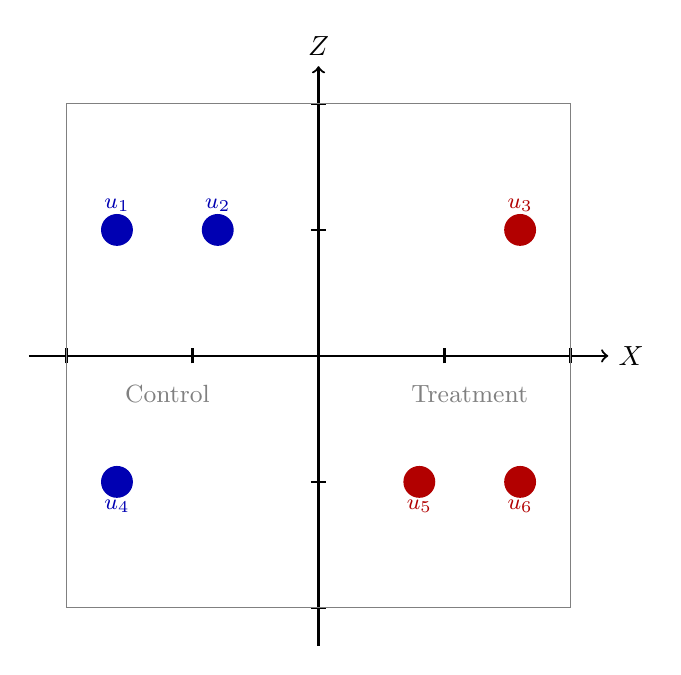
\begin{tikzpicture}[scale=3.2]

	% --- Coordinate axes ---
	\draw[->, thick] (-1.15, 0) -- (1.15, 0) node[right] {$X$};
	\draw[->, thick] (0, -1.15) -- (0, 1.15) node[above] {$Z$};

	% --- Tick marks ---
	\foreach \x in {-1, -0.5, 0.5, 1} {
		\draw[thick] (\x, -0.03) -- (\x, 0.03);
	}
	\foreach \z in {-1, -0.5, 0.5, 1} {
		\draw[thick] (-0.03, \z) -- (0.03, \z);
	}

	% --- Bounding box ---
	\draw[gray, thin] (-1,-1) rectangle (1,1);

	% --- Region labels ---
	\node[gray, font=\small] at (-0.6, -0.15) {Control};
	\node[gray, font=\small] at (0.6, -0.15) {Treatment};

	% --- Sample units ---
	% Top row: z = 0.5
	\fill[blue!70!black] (-0.8, 0.5) circle (1.8pt);
	\fill[blue!70!black] (-0.4, 0.5) circle (1.8pt);
	\fill[red!70!black] (0.8, 0.5) circle (1.8pt);

	% Bottom row: z = -0.5
	\fill[blue!70!black] (-0.8, -0.5) circle (1.8pt);
	\fill[red!70!black] (0.4, -0.5) circle (1.8pt);
	\fill[red!70!black] (0.8, -0.5) circle (1.8pt);

	% --- Unit labels ---
	\node[above=3pt, blue!70!black, font=\footnotesize] at (-0.8, 0.5) {$u_1$};
	\node[above=3pt, blue!70!black, font=\footnotesize] at (-0.4, 0.5) {$u_2$};
	\node[above=3pt, red!70!black, font=\footnotesize] at (0.8, 0.5) {$u_3$};

	\node[below=3pt, blue!70!black, font=\footnotesize] at (-0.8, -0.5) {$u_4$};
	\node[below=3pt, red!70!black, font=\footnotesize] at (0.4, -0.5) {$u_5$};
	\node[below=3pt, red!70!black, font=\footnotesize] at (0.8, -0.5) {$u_6$};

\end{tikzpicture}
\caption{Fixed design with $n = 6$ units. Control units (blue, $x_i < 0$) and treatment units (red, $x_i > 0$) are arranged in two rows at $z = \pm\tfrac{1}{2}$. The design is asymmetric: at $z = \tfrac{1}{2}$, two control units lie near the cutoff while only one treatment unit is available; at $z = -\tfrac{1}{2}$, the pattern reverses.}
\label{fig:design}
\end{figure}

\paragraph{Estimators.}
The local constant estimator assigns equal weight to all units on each side:
\begin{equation}\label{eq:lc_estimator}
	\hat\tau_{\mathrm{lc}} = \underbrace{\tfrac{1}{3}(Y_3 + Y_5 + Y_6)}_{\bar{Y}_T} - \underbrace{\tfrac{1}{3}(Y_1 + Y_2 + Y_4)}_{\bar{Y}_C}.
\end{equation}
This is a $w(X_i)$-only estimator: weights depend only on which side of the cutoff the unit falls.
Its displacement vectors include a cross-row pair $(u_6, u_1)$ with $\Delta_3 = (1.6, -1)$, which compares units at different covariate values.

The segmented estimator adjusts for $Z$ via stratum fixed effects:
\begin{equation}\label{eq:seg_estimator}
	\hat\tau_{\mathrm{seg}} = \frac{1}{2}\Bigl[Y_3 - \tfrac{1}{2}(Y_1 + Y_2)\Bigr] + \frac{1}{2}\Bigl[\tfrac{1}{2}(Y_5 + Y_6) - Y_4\Bigr].
\end{equation}
This is a $w(X_i, Z_i)$ estimator.
All four within-stratum displacement vectors are purely horizontal: $\Delta = (1.6, 0)$ or $(1.2, 0)$.

\paragraph{Worst-case bias under $M_x = 0$.}
Under the anisotropic class with $M_x = 0$, every function is constant in $x$.
The segmented estimator is \emph{exactly unbiased}: all displacements are horizontal, so the $M_z$ bound is orthogonal to the estimation direction.
The local constant estimator has bias $\tfrac{1}{3} M_z$ from the cross pair.

Under the isotropic class, the adversary can tilt the function into $x$ at the expense of $z$-variation, so the direction-specific information $M_x = 0$ cannot be exploited.
The gap between the two classes is the cost of coupling.

\commentT{Conjecture: $\mathcal{F}^{\mathrm{iso}} \subseteq \mathcal{F}^P$ in the tuple space.  The pooled class's derived bound is $\ell_1$-type ($M_x^P = M_x + M_z L$), while the isotropic coupling is $\ell_2$-type.  Since $\norm{v}_1 \geq \norm{v}_2$ for all $v$, this should follow.  To do: formalize.}

\commentT{Compute explicit worst-case bias for both estimators under iso with $M_x = 0$ to quantify the gap.}


%%%%%%%%%%%%%%%%%%%%%%%%%%%%%%%%%%%%%%%%%%%%%%%%%%%%%%%%%%%%
\section{Technical Results}\label{sec:technical}
%%%%%%%%%%%%%%%%%%%%%%%%%%%%%%%%%%%%%%%%%%%%%%%%%%%%%%%%%%%%


\subsection{Support Functions and Gradient-Constrained Classes}\label{sec:technical:support}

\begin{definition}[Gradient-constrained smoothness class]\label{def:gradient_class}
	Let $\mathcal{C} \subset \mathbb{R}^2$ be a compact, convex set containing the origin.
	The gradient-constrained smoothness class induced by $\mathcal{C}$ is
	\begin{equation*}
		\mathcal{F}(\mathcal{C}) \defeq \bigl\{ f : \mathbb{R}^2 \to \mathbb{R} \;\big|\; \nabla f(x,z) \in \mathcal{C} \;\; \text{for all } (x,z) \bigr\}.
	\end{equation*}
\end{definition}

The \emph{support function} of $\mathcal{C}$ is
\begin{equation*}
	h_{\mathcal{C}}(v) = \sup\bigl\{ \langle u, v \rangle : u \in \mathcal{C} \bigr\}, \qquad v \in \mathbb{R}^d.
\end{equation*}
By standard convex duality, $\mathcal{C}$ is recovered from $h_{\mathcal{C}}$:
\begin{equation}\label{eq:C_from_h}
	\mathcal{C} = \bigl\{ u \in \mathbb{R}^d : \langle u, v \rangle \leq h_{\mathcal{C}}(v) \text{ for all } v \in \mathbb{R}^d \bigr\}.
\end{equation}

\begin{lemma}[Gradient constraint via support function]\label{lem:gradient_support}
	Let $\mathcal{C} \subset \mathbb{R}^d$ be compact and convex with $0 \in \mathcal{C}$.
	Then $\nabla f(x) \in \mathcal{C}$ for all $x$ if and only if
	\begin{equation}\label{eq:dir_deriv_bound}
		D_v f(x) \leq h_{\mathcal{C}}(v) \qquad \text{for all } x \text{ and all } v \in \mathbb{R}^d.
	\end{equation}
\end{lemma}

\begin{proof}
	If $\nabla f(x) \in \mathcal{C}$, then $D_v f(x) = \langle \nabla f(x), v \rangle \leq \sup_{u \in \mathcal{C}} \langle u, v \rangle = h_{\mathcal{C}}(v)$.
	Conversely, if \eqref{eq:dir_deriv_bound} holds for all $v$, then $\langle \nabla f(x), v \rangle \leq h_{\mathcal{C}}(v)$ for all $v$, which by \eqref{eq:C_from_h} implies $\nabla f(x) \in \mathcal{C}$.
\end{proof}

\begin{lemma}[Direction-dependent Lipschitz property]\label{lem:lipschitz}
	If $f \in \mathcal{F}(\mathcal{C})$, then for any two points $x, x'$,
	\begin{equation}\label{eq:lipschitz_onesided}
		f(x') - f(x) \leq h_{\mathcal{C}}(x' - x).
	\end{equation}
	If in addition $\mathcal{C}$ is symmetric ($\mathcal{C} = -\mathcal{C}$), then $\abs{f(x') - f(x)} \leq h_{\mathcal{C}}(x' - x)$.
	The bound is tight: $f^*(x) = h_{\mathcal{C}}(x) \in \mathcal{F}(\mathcal{C})$ achieves $f^*(d) - f^*(0) = h_{\mathcal{C}}(d)$.
\end{lemma}

\begin{proof}
	By the fundamental theorem of calculus,
	\begin{equation*}
		f(x') - f(x) = \int_0^1 \langle \nabla f(x + t(x'-x)),\, x' - x \rangle \, dt \leq \int_0^1 h_{\mathcal{C}}(x' - x) \, dt = h_{\mathcal{C}}(x' - x),
	\end{equation*}
	using \cref{lem:gradient_support}.
	For tightness: $h_{\mathcal{C}}$ is convex and positively homogeneous, hence differentiable a.e.\ with $\nabla h_{\mathcal{C}}(x) \in \mathcal{C}$ (as a subgradient), so $f^* = h_{\mathcal{C}} \in \mathcal{F}(\mathcal{C})$.
\end{proof}

The support function $h_{\mathcal{C}}(d)$ has a concrete geometric interpretation: it is the maximum change in $f$ over the displacement $d$, given that the gradient must lie in $\mathcal{C}$.
The adversary picks the gradient $g \in \mathcal{C}$ that is most aligned with $d$, achieving $\langle g, d \rangle = \|g\| \|d\| \cos\theta$.
The displacement's \emph{direction} selects which part of $\partial\mathcal{C}$ the adversary uses; its \emph{magnitude} determines how far the function can ramp.
For the rectangle, the maximizer is always a corner: $g^* = (M_x \sign(d_1),\, M_z \sign(d_2))$, giving $h_{\mathcal{C}_s}(d) = M_x\abs{d_1} + M_z\abs{d_2}$.
The absolute gradient components are always $(M_x, M_z)$ regardless of the displacement direction --- each coordinate uses its full budget independently, just as in the univariate case.
For the disk, the maximizer rotates with the displacement: $g^* = R \cdot d / \|d\|$, giving $h_{B_2}(d) = R\|d\|$.
A horizontal displacement activates gradient $(R, 0)$; a diagonal displacement activates $(R/\sqrt{2},\, R/\sqrt{2})$.
The gradient budget is reallocated across coordinates depending on the direction --- this is the geometric content of coupling.
In an estimation problem with weights $w = (w_1, \ldots, w_n)$ and displacements $\Delta_i$ from the target to each design point, the worst-case bias is $\sum_i \abs{w_i}\, h_{\mathcal{C}}(\Delta_i)$: each displacement contributes its own support function evaluation, and the total bias is the sum over the entire sample.

\subsection{Coordinate Decomposition and Coupling in Proofs}\label{sec:technical:decomposition}

The bound in \cref{lem:lipschitz} specializes differently for the two constraint sets, and the difference reveals how coupling enters at the proof level.

\paragraph{Anisotropic class (rectangle).}
The constraint set is the product $[-M_x, M_x] \times [-M_z, M_z]$, so the partial derivative bounds are independent: knowing $\abs{\partial f / \partial x}$ places no restriction on $\abs{\partial f / \partial z}$.
To bound $f(x', z') - f(x, z)$, decompose the path into coordinate segments:
\begin{equation}\label{eq:ftc_aniso}
	f(x', z') - f(x, z) = \int_x^{x'} \frac{\partial f}{\partial x}(t, z)\, dt + \int_z^{z'} \frac{\partial f}{\partial z}(x', s)\, ds.
\end{equation}
Each integral is bounded independently: the first by $M_x\abs{x' - x}$, the second by $M_z\abs{z' - z}$.
The two bounds do not interact --- the worst case for the horizontal leg and the worst case for the vertical leg are achieved simultaneously, because the constraint set is a Cartesian product.
The resulting bound is
\begin{equation*}
	f(x', z') - f(x, z) \leq M_x\abs{x' - x} + M_z\abs{z' - z} = h_{\mathrm{rect}}(x' - x, z' - z).
\end{equation*}

\paragraph{Isotropic class (disk).}
The constraint $\norm{\nabla f}_2 \leq R$ couples the partials: if $\abs{\partial f / \partial x}$ is close to $R$, then $\abs{\partial f / \partial z}$ must be close to zero.
The coordinate decomposition \eqref{eq:ftc_aniso} is no longer useful, because bounding each partial at $R$ separately would give the rectangle bound $R\abs{\Delta x} + R\abs{\Delta z}$ --- an overestimate that ignores the coupling.
Instead, the proof takes the straight-line path and bounds the directional derivative jointly via Cauchy--Schwarz:
\begin{equation*}
	f(x', z') - f(x, z) = \int_0^1 \langle \nabla f(\gamma(t)),\, (\Delta x, \Delta z) \rangle\, dt \leq \norm{\nabla f}_2 \norm{(\Delta x, \Delta z)}_2 \leq R\sqrt{\Delta x^2 + \Delta z^2} = h_{\mathrm{disk}}(\Delta x, \Delta z).
\end{equation*}
To see this concretely, parameterize the straight line from $(x, z)$ to $(x', z')$ as $\gamma(t) = (x + t\Delta x,\; z + t\Delta z)$ with $\Delta x = x' - x$ and $\Delta z = z' - z$.
The chain rule gives:
\begin{equation*}
	\frac{d}{dt}f(\gamma(t)) = \frac{\partial f}{\partial x}(\gamma(t))\cdot \frac{d\gamma_1}{dt} + \frac{\partial f}{\partial z}(\gamma(t))\cdot \frac{d\gamma_2}{dt} = \frac{\partial f}{\partial x}(\gamma(t))\cdot \Delta x + \frac{\partial f}{\partial z}(\gamma(t))\cdot \Delta z,
\end{equation*}
where $\frac{d\gamma_1}{dt} = \Delta x$ and $\frac{d\gamma_2}{dt} = \Delta z$ are constants (the velocity of the straight line).
Integrating from $t = 0$ to $t = 1$ recovers $f(x', z') - f(x, z)$:
\begin{equation*}
	f(x', z') - f(x, z) = \int_0^1 \left[ \frac{\partial f}{\partial x}(\gamma(t))\, \Delta x + \frac{\partial f}{\partial z}(\gamma(t))\, \Delta z \right] dt \leq \sqrt{\left(\frac{\partial f}{\partial x}\right)^2 + \left(\frac{\partial f}{\partial z}\right)^2}\; \sqrt{\Delta x^2 + \Delta z^2} \leq R\sqrt{\Delta x^2 + \Delta z^2}.
\end{equation*}
The coordinates are never separated.
The worst-case gradient aligns with the displacement direction: for a displacement mostly in $x$, the adversary concentrates the entire gradient budget into $\partial f / \partial x$, setting $\partial f / \partial z \approx 0$.

\paragraph{Consequence for estimation.}
A linear estimator $\hat{L} = \sum_i w_i Y_i$ targeting $f(x_0)$ has worst-case bias $\sum_i \abs{w_i}\, h_{\mathcal{C}}(x_i - x_0)$.
For the segmented estimator, all displacements are horizontal ($\Delta z_i = 0$), so:
\begin{alignat*}{2}
	&\text{Rectangle:} &\quad \wcb &= \textstyle\sum_i \abs{w_i}\, M_x\abs{\Delta x_i}, \\
	&\text{Disk:} &\quad \wcb &= \textstyle\sum_i \abs{w_i}\, R\abs{\Delta x_i}.
\end{alignat*}
Under the rectangle, the $M_z$ bound is \emph{stranded}: it cannot contribute to bias along horizontal displacements.
Under the disk, the adversary reallocates the freed $z$-budget into $x$, inflating the effective bound from $M_x$ to $R = \sqrt{M_x^2 + M_z^2} > M_x$.
This is the proof-level manifestation of coupling: the isotropic constraint prevents the analyst from exploiting the per-direction structure of the displacements.


\subsection{Modulus of Continuity}\label{sec:technical:modulus}

In real analysis, the modulus of continuity of a function class $\mathcal{F}$ is
\begin{equation*}
	\omega(\delta; \mathcal{F}) = \sup\bigl\{ \abs{f(x) - f(y)} : \abs{x - y} \leq \delta,\; f \in \mathcal{F} \bigr\}.
\end{equation*}
It measures worst-case oscillation over $\delta$-intervals: for Lipschitz-$M$ functions, $\omega(\delta) = M\delta$.

The statistical modulus \parencite{donoho_statistical_1994,armstrong_optimal_2018} generalizes this.
Let $\mathcal{F}$ be convex, $K$ a linear observation operator, $Lf$ a linear functional.
We observe $Y = Kf + \sigma\varepsilon$.
The single-class modulus (for centrosymmetric $\mathcal{F}$) is
\begin{equation}\label{eq:modulus_single}
	\omega(\delta; \mathcal{F}) = \sup\bigl\{ 2Lf : \norm{Kf} \leq \delta/2,\; f \in \mathcal{F} \bigr\}.
\end{equation}
The parallel is exact: $\abs{x - y} \leq \delta$ becomes $\norm{K(g-f)} \leq \delta$ (distance in the data), and $\abs{f(x) - f(y)}$ becomes $Lg - Lf$ (gap in the target).
By Theorem~3.1 of \textcite{armstrong_optimal_2018}, the minimax risk is governed by $\omega$: all optimal bias--variance tradeoffs are parameterized by the modulus.

\begin{corollary}[Modulus as a functional of the support function]\label{cor:modulus_functional}
	For a gradient-constrained class $\mathcal{F}(\mathcal{C})$, the modulus of continuity depends on $\mathcal{C}$ only through its support function $h_{\mathcal{C}}$:
	\begin{equation*}
		\omega(\delta; \mathcal{F}(\mathcal{C})) = \Omega(\delta,\, h_{\mathcal{C}}).
	\end{equation*}
\end{corollary}

\begin{proof}
	By \cref{lem:gradient_support}, $f \in \mathcal{F}(\mathcal{C})$ if and only if $D_v f(x) \leq h_{\mathcal{C}}(v)$ for all $x, v$.
	Substituting into \eqref{eq:modulus_single}, the constraint on $f$ is expressed entirely in terms of $h_{\mathcal{C}}$.
	Since $h_{\mathcal{C}}$ determines $\mathcal{C}$ uniquely (by \eqref{eq:C_from_h}), the modulus is a functional of $h_{\mathcal{C}}$.
\end{proof}


\subsection{Worst-Case Bias}\label{sec:technical:wcb}

\begin{proposition}[Worst-case bias over $\mathcal{F}(\mathcal{C})$]\label{prop:wcb}
	Let $\hat{L} = \sum_{i} w_i Y_i$ be a linear estimator of $Lf = f(x_0)$, with $\sum_i w_i = 1$.
	Then the worst-case bias over $\mathcal{F}(\mathcal{C})$ is
	\begin{equation}\label{eq:wcb_general}
		\wcb_{\mathcal{F}(\mathcal{C})}(\hat{L}) \defeq \sup_{f \in \mathcal{F}(\mathcal{C})} \bigl( \E[\hat{L}] - f(x_0) \bigr) = \sum_{i=1}^n w_i \, h_{\mathcal{C}}(x_i - x_0),
	\end{equation}
	where the supremum is attained by $f^*(x) = h_{\mathcal{C}}(x - x_0)$.

	For symmetric $\mathcal{C}$, the maximum absolute bias is
	\begin{equation}\label{eq:wcb_abs}
		\sup_{f \in \mathcal{F}(\mathcal{C})} \abs{\E[\hat{L}] - f(x_0)} = \sum_{i=1}^n \abs{w_i} \, h_{\mathcal{C}}(x_i - x_0).
	\end{equation}
\end{proposition}

\begin{proof}
	For any $f \in \mathcal{F}(\mathcal{C})$,
	$\E[\hat{L}] - f(x_0) = \sum_i w_i (f(x_i) - f(x_0))$.
	By \cref{lem:lipschitz}, $f(x_i) - f(x_0) \leq h_{\mathcal{C}}(x_i - x_0)$.
	The bound is attained by $f^*(x) = h_{\mathcal{C}}(x - x_0) \in \mathcal{F}(\mathcal{C})$.
	Since $h_{\mathcal{C}}(x_i - x_0) \geq 0$, $f^*$ achieves the upper bound at every observation when all $w_i \geq 0$.

	\commentT{The absolute value formula \eqref{eq:wcb_abs} needs revision for mixed-sign weights.  The argument requires a single $f$ to simultaneously achieve $+h_{\mathcal{C}}$ at positive-weight and $-h_{\mathcal{C}}$ at negative-weight observations, but the inter-observation Lipschitz constraint prevents this in general.  Counterexample: $w_1 = 2$ at $x_1 = 1$, $w_2 = -1$ at $x_2 = 2$, $x_0 = 0$, Lipschitz $M = 1$; formula gives $4$, actual wcb is $2$.  Three options: (1) restrict to $w_i \geq 0$, (2) state as upper bound, (3) solve the constrained LP over $\Delta_i = f(x_i) - f(x_0)$.}
\end{proof}

Specializing to the two constraint sets:
\begin{align}
	\wcb_{\mathrm{rect}}(\hat{L}) &= \sum_{i} \abs{w_i} \bigl( M_x \abs{x_i - x_0^{(1)}} + M_z \abs{z_i - x_0^{(2)}} \bigr), \label{eq:wcb_rect} \\
	\wcb_{\mathrm{disk}}(\hat{L}) &= \sum_{i} \abs{w_i} \, R \sqrt{(x_i - x_0^{(1)})^2 + (z_i - x_0^{(2)})^2}. \label{eq:wcb_disk}
\end{align}
The rectangle's worst-case bias decomposes additively; the disk's couples the directions through $\ell_2$.


\subsection{Monotonicity of the Modulus}\label{sec:technical:monotonicity}

\begin{theorem}[Monotonicity]\label{thm:monotonicity}
	Let $\mathcal{C}_1 \subseteq \mathcal{C}_2$ be compact convex sets.
	Then $\omega(\delta; \mathcal{F}(\mathcal{C}_1)) \leq \omega(\delta; \mathcal{F}(\mathcal{C}_2))$ for all $\delta > 0$.
\end{theorem}

\begin{proof}
	$\mathcal{C}_1 \subseteq \mathcal{C}_2$ implies $\mathcal{F}(\mathcal{C}_1) \subseteq \mathcal{F}(\mathcal{C}_2)$.
	The modulus \eqref{eq:modulus_single} is a supremum over $\mathcal{F}$; enlarging the feasible set cannot decrease the value.
\end{proof}

\begin{theorem}[Strict monotonicity]\label{thm:strict_monotonicity}
	Let $\mathcal{C}_1 \subsetneq \mathcal{C}_2$ with $\mathcal{C}_1$ having nonempty interior.
	Then $\omega(\delta; \mathcal{F}(\mathcal{C}_1)) < \omega(\delta; \mathcal{F}(\mathcal{C}_2))$ for all $\delta > 0$.
\end{theorem}

\begin{proof}[Proof sketch]
	Since $\mathcal{C}_1 \subsetneq \mathcal{C}_2$, there exists $u^* \in \mathcal{C}_2 \setminus \mathcal{C}_1$.
	By the separation theorem, $h_{\mathcal{C}_2}(v^*) > h_{\mathcal{C}_1}(v^*)$ for some direction $v^*$.
	The modulus-achieving function for $\mathcal{F}(\mathcal{C}_1)$ can be perturbed to tilt the gradient toward $u^*$, remaining in $\mathcal{F}(\mathcal{C}_2)$ while strictly increasing $Lf$.

	\commentT{This proof sketch needs to be made rigorous.  The key step is constructing a perturbation that exploits the extra gradient freedom in $\mathcal{C}_2 \setminus \mathcal{C}_1$ to strictly increase $Lf$ without violating $\norm{Kf} \leq \delta/2$.  Core open problem.}

	\commentT{The theorem as stated is too strong.  Strict set inclusion $\mathcal{C}_1 \subsetneq \mathcal{C}_2$ (both compact) guarantees $h_{\mathcal{C}_1}(v^*) < h_{\mathcal{C}_2}(v^*)$ for some direction $v^*$ (by the support function's uniqueness for compact convex sets).  However, strict inequality of the modulus requires that $v^*$ aligns with a displacement direction $x_i - x_0$ that the estimation problem actually uses.  If the design has no observations with displacement component in the $v^*$ direction, the extra freedom in $\mathcal{C}_2 \setminus \mathcal{C}_1$ is invisible to the modulus.  The correct condition is: $h_{\mathcal{C}_1}(v) < h_{\mathcal{C}_2}(v)$ for some $v$ in the set of displacement directions relevant to $(L, K)$.  In the bivariate case, this fails only if all design points and the target lie on the same line in the covariate space --- e.g., all units share the same $Z$-value, so all displacements are purely horizontal.  This is the degenerate case of complete $Z$-invariance in the design.  Whenever $Z$ has variation (observations at different covariate values), the displacement vectors span $\mathbb{R}^2$, and any strict difference between $h_{\mathcal{C}_1}$ and $h_{\mathcal{C}_2}$ in any direction is exploitable.  Note also: compactness is doing real work here.  For non-compact sets (e.g.\ $\mathcal{C}_1 = \mathrm{int}(\mathcal{C}_2)$), strict set inclusion holds but the support functions are identical, so the moduli coincide trivially.  Compactness prevents this by ensuring the support function uniquely determines the set.}
\end{proof}

\begin{corollary}[Strict improvement from anisotropic class]\label{cor:strict_improvement}
	For any $M_x, M_z > 0$, with $R = \sqrt{M_x^2 + M_z^2}$,
	\begin{equation*}
		\omega\bigl(\delta; \mathcal{F}(\mathcal{C}_{\mathrm{rect}})\bigr) < \omega\bigl(\delta; \mathcal{F}(\mathcal{C}_{\mathrm{disk}})\bigr) \qquad \text{for all } \delta > 0.
	\end{equation*}
\end{corollary}

\begin{proof}
	$\mathcal{C}_{\mathrm{rect}} \subsetneq \mathcal{C}_{\mathrm{disk}}$: the corners $(\pm M_x, \pm M_z)$ lie on the disk boundary, but $(R, 0) \in \mathcal{C}_{\mathrm{disk}} \setminus \mathcal{C}_{\mathrm{rect}}$ since $R > M_x$.
	Apply \cref{thm:strict_monotonicity}.
\end{proof}


\subsection{Z-Balance and the Necessity of Covariate Variation}\label{sec:technical:zbalance}

\begin{definition}[$Z$-balanced design]\label{def:z_balanced}
	A fixed design $\{(x_i, z_i)\}_{i=1}^n$ is \emph{$Z$-balanced} if, on each side of the cutoff, the multiset of $x$-positions is identical across all $z$-strata.
	That is, for each treatment status $d \in \{0,1\}$, the conditional empirical distribution of $x_i$ given $z_i = z$ and $D_i = d$ does not depend on $z$.
\end{definition}

\begin{proposition}[$Z$-imbalance is necessary for strict improvement from covariate adjustment]\label{prop:z_imbalance}
	Consider a fixed design $\{(x_i, z_i)\}_{i=1}^n$ with homoscedastic errors and target $\tau$ at the cutoff.
	\begin{enumerate}
		\item If the design is $Z$-balanced, the local constant and segmented estimators coincide: $\hat\tau_{\mathrm{lc}} = \hat\tau_{\mathrm{seg}}$.
		Covariate adjustment does not reduce worst-case bias under any primitive-consistent $\mathcal{C}$.
		\item If the design is $Z$-imbalanced and $M_z > 0$, the segmented estimator has strictly lower worst-case bias than the local constant estimator under $\mathcal{F}(\mathcal{C}_{\mathrm{rect}})$.
	\end{enumerate}
\end{proposition}

\begin{proof}[Proof sketch]
	(1) Under $Z$-balance, each $z$-stratum contains the same $x$-positions on each side of the cutoff.
	The segmented estimator computes within-stratum treatment effects using identical $x$-pairs and averages across strata; this coincides with the local constant estimator, which pools across strata with equal weights.
	Since the estimators coincide, their worst-case biases are identical --- covariate adjustment is redundant.

	(2) Under $Z$-imbalance, the local constant estimator necessarily makes cross-stratum comparisons: there exist paired units $(x_i, z_i)$ and $(x_j, z_j)$ with $z_i \neq z_j$ on opposite sides of the cutoff.
	The displacement $d = (x_i - x_j,\, z_i - z_j)$ has $\Delta z \neq 0$, contributing $M_z\abs{\Delta z}$ to the worst-case bias under $h_{\mathrm{rect}}$.
	The segmented estimator avoids these cross-stratum displacements entirely: all its within-stratum displacement vectors satisfy $\Delta z = 0$, so the $M_z$ bound is stranded.
\end{proof}

\begin{remark}
	$Z$-balance is the design-level condition under which the $z$-direction of the support function is irrelevant to the minimax problem.
	It arises only under complete $Z$-degeneracy: the covariate provides no additional design variation beyond what is already present in the running variable.
	This is precisely the condition under which covariate adjustment is redundant --- the estimator cannot exploit $Z$ because $Z$ carries no information not already encoded in the $X$-design.
	In any design with genuine $Z$-variation (different $x$-configurations across $z$-strata), the segmented estimator strictly outperforms the local constant under the anisotropic class.
\end{remark}

\begin{remark}[The cost of isotropy under $Z$-balance]\label{rem:isotropy_zbalance}
	Under $Z$-balance, the worst-case bias of the local constant estimator under $\mathcal{C}_s$ is purely in the $x$-direction: the $z$-variation cancels across strata, stranding the $M_z$ budget.
	The worst-case bias is $M_x \sum_i \abs{w_i} \abs{\Delta x_i}$.
	Under the isotropic disk $B_2(R)$ with $R = \sqrt{M_x^2 + M_z^2}$, the adversary reallocates the entire gradient budget into $x$, giving worst-case bias $R \sum_i \abs{w_i} \abs{\Delta x_i}$.
	The disk overestimates the worst-case bias by the inflation factor $R / M_x = \sqrt{1 + M_z^2 / M_x^2}$, which equals $\sqrt{2}$ in the symmetric case $M_x = M_z$.
	This is the cost of encoding the primitive information inefficiently: the separable class correctly identifies the $M_z$ budget as irrelevant under $Z$-balance, while the isotropic class makes it transferable to $M_x$, producing a worst-case bias bound that is too large by a factor of $\sqrt{2}$.

	In the degenerate case where all units share the same covariate value $z_i = z_0$, the argument extends beyond the local constant estimator: \emph{every} linear estimator has purely horizontal displacement vectors, so the worst-case bias under the disk exceeds that under the rectangle by the factor $R / M_x$ regardless of the choice of weights.
	The minimax risk itself is inflated by this factor, since the modulus of continuity sees only the restriction of $f$ to the line $z = z_0$, where the effective Lipschitz constant is $M_x$ under the rectangle versus $R$ under the disk.
\end{remark}

\begin{remark}[Modulus separation for point evaluation $\tau(c, z)$]\label{rem:modulus_separation}
	Consider the point functional $L(f) = \tau(c, z_0) = f(c^+, z_0) - f(c^-, z_0)$ for a fixed covariate value $z_0$, estimated from design points $\{(x_i, z_i)\}_{i=1}^n$.
	The displacement vectors from the target $(c, z_0)$ to the design points are $\Delta_i = (x_i - c,\, z_i - z_0)$, which are fixed by the design.
	The modulus of continuity $\omega(\delta; L, K, \mathcal{F}(\mathcal{C}))$ depends on the constraint set $\mathcal{C}$ through the directions these displacements activate:
	\begin{enumerate}
		\item \emph{Monotonicity.}  $\mathcal{C}_s \subseteq B_2(R)$ implies $\mathcal{F}(\mathcal{C}_s) \subseteq \mathcal{F}(B_2(R))$, hence $\omega(\delta; \mathcal{C}_s) \leq \omega(\delta; B_2(R))$ for all $\delta$.  The minimax risk under the separable class is weakly smaller.
		\item \emph{Equality condition.}  The moduli coincide if and only if the modulus-attaining function pair uses gradients exclusively in the direction $(\pm M_x, \pm M_z)$ --- the corners of $\mathcal{C}_s$, which lie on $\partial B_2(R)$.  At these points the two constraint sets agree.
		\item \emph{Strict inequality.}  If even a single displacement $\Delta_i$ is not proportional to $(M_x, M_z)$, then $h_{B_2}(\Delta_i) > h_{\mathcal{C}_s}(\Delta_i)$: the disk allows the function to decay faster from the target to that design point than the rectangle does, using gradients outside $\mathcal{C}_s$.  That observation becomes less informative under the disk, and the adversary can hide a larger value at $x_0$.  Since the modulus is a supremum over functions satisfying the data constraint at all design points simultaneously, one misaligned displacement suffices: $\omega(\delta; B_2(R)) > \omega(\delta; \mathcal{C}_s)$.
		\item \emph{Maximum gap.}  When displacement is purely along $x$ (i.e., $z_i = z_0$ for all $i$), the disk allows gradient $R$ while the rectangle allows $M_x$.  The inflation factor is $R / M_x = \sqrt{1 + M_z^2 / M_x^2}$, which equals $\sqrt{2}$ in the symmetric case.
		\item \emph{Design determines the gap.}  The displacement vectors $\Delta_i$ are determined by the design $K$.  They determine which part of the constraint set boundary the modulus exploits, placing the inflation factor in $[1,\, \sqrt{1 + M_z^2 / M_x^2}]$.
	\end{enumerate}
	In particular, the minimax risk under $\mathcal{C}_s$ is always weakly smaller, and strictly smaller for any design whose displacement vectors do not all align with the slope $M_z / M_x$.
	The bias inflation can reach $\sqrt{2}$ (symmetric case) when the design generates purely horizontal displacements.
\end{remark}

\begin{remark}[Bias inflation on the equispaced lattice]\label{rem:lattice_inflation}
	For a fixed linear estimator with weights $w = (w_1, \ldots, w_n)$ targeting $f(0,0)$, the worst-case bias under constraint set $\mathcal{C}$ is $\sum_i \abs{w_i}\, h_{\mathcal{C}}(\Delta_i)$, where $\Delta_i = (x_i, z_i)$ is the displacement from the target to design point $i$.
	The bias inflation from using the disk instead of the rectangle is
	\begin{equation*}
		\rho_n \defeq \frac{\sum_i \abs{w_i}\, h_{B_2}(\Delta_i)}{\sum_i \abs{w_i}\, h_{\mathcal{C}_s}(\Delta_i)} = \frac{\sum_i \abs{w_i}\, R \norm{\Delta_i}_2}{\sum_i \abs{w_i}\, (M_x\abs{x_i} + M_z\abs{z_i})}.
	\end{equation*}
	Consider the equispaced lattice design on $[-1,1]^2$ with $(n+1)^2$ design points $\{(x_i, z_j)\}$ where $x_i = -1 + 2i/n$, $z_j = -1 + 2j/n$ for $i, j = 0, \ldots, n$, target at the origin, and equal weights.
	The ratio $\rho_n$ is exactly computable for any $n$ and converges as $n \to \infty$ to
	\begin{equation*}
		\rho = \frac{R \cdot \tfrac{\sqrt{2} + \ln(1 + \sqrt{2})}{3}}{\tfrac{M_x + M_z}{2}},
	\end{equation*}
	using $\int_{[-1,1]^2} \sqrt{x^2 + z^2}\, dx\, dz / 4 = (\sqrt{2} + \ln(1+\sqrt{2}))/3 \approx 0.765$.
	Convergence is fast: $\rho_n$ is within $0.001$ of the limit for $n \geq 50$ (see \texttt{code/01\_lattice\_bias\_inflation.R}).

	\emph{Symmetric case} ($M_x = M_z$, $R = M_x\sqrt{2}$): $\rho \approx 1.082$ --- $8\%$ inflation, against a maximum of $\sqrt{2} \approx 1.414$.
	The longest displacements point toward the corners of $[-1,1]^2$ at slope $1$, which coincides with the slope $M_z / M_x = 1$ where $\mathcal{C}_s$ and $B_2(R)$ agree.

	\emph{Moderately asymmetric case} ($M_z = 2 M_x$, $R = M_x\sqrt{5}$): $\rho \approx 1.141$ --- $14\%$ inflation, against a maximum of $\sqrt{5} \approx 2.236$.
	The agreement slope shifts to $\arctan(2) \approx 63°$, while the longest displacements still point at $45°$; the angular mismatch activates directions where $B_2(R) \supsetneq \mathcal{C}_s$.

	\emph{Strongly asymmetric case} ($M_z = 5 M_x$, $R = M_x\sqrt{26}$): $\rho \approx 1.301$ --- $30\%$ inflation, against a maximum of $\sqrt{26} \approx 5.099$.
	The agreement direction is now $\arctan(5) \approx 79°$, nearly vertical, while the design geometry remains isotropic at $45°$.

	The general pattern: the bias inflation grows with the angular gap between the agreement direction $\arctan(M_z / M_x)$ and the dominant displacement direction of the design.
\end{remark}

\begin{remark}[Bias inflation under random designs]\label{rem:uniform_inflation}
	Under a random design $(x_i, z_i) \iid f(x, z)$ with equal weights, $\rho_n$ converges by the law of large numbers to the same limit as the lattice.
	More generally, the bias inflation under a random design with joint density $f(x, z)$ is a \emph{density-weighted mean width ratio}: the pointwise support function ratio $r(\Delta_i)$ from \cref{def:sfr} is averaged over the design distribution, with each direction weighted by the displacement magnitude and the density.
	The design geometry and the constraint set geometry interact: the inflation is largest when the density concentrates mass on displacements along the coordinate axes (where $r$ is maximized) and smallest when it concentrates mass near the slope $M_z / M_x$ (where $r = 1$).
\end{remark}

\commentT{Decision-theoretic framing of the weak inequality.  The result $R^*(\mathcal{F}(\mathcal{C}_s), K) \leq R^*(\mathcal{F}(B_2(R)), K)$ for all designs $K$ is a \emph{dominance} result in the decision-theoretic sense (Blackwell-style): the separable class weakly dominates the disk across all designs.  The equality set is fully characterized: equality holds if and only if all displacement vectors $\Delta_i$ from the target to the design points are proportional to $(\pm M_x, \pm M_z)$ --- the corners of $\mathcal{C}_s$ where the two constraint sets agree.  This is a knife-edge condition: under any continuous design distribution with $f(x,z) > 0$, it holds with probability zero.  The weak inequality with characterized equality is the standard form for such results; Blackwell's theorem itself is a weak inequality with a characterized equality case.  The contribution is the characterization --- how convex smoothness classes encode assumptions on the regression function --- not the magnitude of the inflation.

	The lattice examples in \cref{rem:lattice_inflation} are \emph{integrated risk} computations in the following sense: $\rho_n$ averages the deterministic support-function ratio over the design points, producing a summary of the AK fixed-design risk across the lattice.  This is a descriptive summary of the design-dependent risk, not random-design inference.  The paper stays entirely within the AK fixed-design framework; no asymptotic equivalence results are invoked.}

\commentT{Conditions for strict modulus separation between rectangle and disk.  By \cref{lem:ratio_range}, the pointwise support function ratio $r(v) = h_{\mathrm{disk}}(v) / h_{\mathrm{rect}}(v)$ equals 1 only when $v \propto (M_x, M_z)$; in all other directions $r(v) > 1$.  The modulus under the disk is therefore strictly larger than under the rectangle unless the worst-case function generates bias exclusively along the direction $(M_x, M_z)$.  This requires all relevant displacement directions in the estimation problem to align with $(M_x, M_z)$, i.e., $\Delta z_i / \Delta x_i = M_z / M_x$ for every observation --- all design points lie on a single ray through the target at slope $M_z / M_x$.  This is a knife-edge condition that fails whenever the design has any $z$-variation not perfectly tracking this slope.  The single-line case ($z_i = z_0$ for all $i$) is the opposite extreme: all displacements are horizontal, the direction where $r(v) = R / M_x$ is maximized.  This connects the pointwise ratio lemma to the modulus: the lemma identifies where disk and rectangle agree and disagree, the design determines which directions the modulus exploits.  To do: formalize the condition on displacement directions that guarantees strict modulus separation and determine whether general $Z$-balance (not just the single-line case) suffices for all minimax-optimal estimators.}

\commentT{Under a random design drawn from any continuous joint density $f(x,z) > 0$, exact $Z$-balance (identical $x$-realizations across $z$-strata) is an event of probability zero.  Therefore, with probability 1 over the random design, the $Z$-imbalance condition of \cref{prop:z_imbalance} holds, and covariate adjustment yields a strict improvement.  The strict improvement is generic: it holds almost surely without needing to verify the imbalance condition.  The fixed-design result (\cref{prop:z_imbalance}) identifies the knife-edge pathology; the random-design perspective shows it never occurs in practice with continuous covariates.  This could be formalized as a corollary: under any DGP with continuous $(X, Z)$ and $f_{X,Z} > 0$, $R^*_{\mathrm{seg}} < R^*_{\mathrm{lc}}$ almost surely.}

\commentT{Practical diagnostic: for a given fixed design, the $Z$-balance condition is directly verifiable.  Define a \emph{$Z$-imbalance statistic} that quantifies the deviation from balance and gauges the potential gain from covariate adjustment.  Three approaches at different levels of generality:

	(1) \emph{Bias decomposition under the relevant function class.}  In existing univariate RDD designs, practitioners impose a joint smoothness bound (typically isotropic or elliptic --- a convex class inscribing the anisotropic rectangle).  Under any such class, the worst-case bias of the LC estimator decomposes into an $x$-component and a $z$-component.  The $z$-component, $M_z \sum_i |w_i^{\mathrm{lc}}| |\Delta z_i|$ under the rectangle, is what covariate adjustment can eliminate.  This is directly computable for any design and any convex constraint set, and is interpretable in worst-case bias units.

	(2) \emph{Dependence measures.}  Any measure of dependence between $X$ and $Z$ conditional on treatment status ($X \perp Z \mid D$ is the continuous $Z$-balance condition).  Linear correlation $|\mathrm{Corr}(X_i, Z_i \mid D_i)|$ is a first step but may miss nonlinear dependence.

	(3) \emph{Propensity score variation} (most promising).  The conditional propensity score $e(z) = P(D_i = 1 \mid Z_i = z)$ within the bandwidth is the natural sufficient statistic.  It aggregates the conditional density $f_{X|Z}(x \mid z)$ within the bandwidth into a single scalar at each covariate value.  Constant $e(z) = e$ corresponds to exact $Z$-balance: the treated/control mix does not depend on the covariate.  Variation in $e(z)$ is $Z$-imbalance: at some covariate values there are proportionally more treated observations, creating the cross-stratum displacements that covariate adjustment eliminates.  This is easy to estimate (local logistic regression of $D_i$ on $Z_i$, or a kernel smoother), directly interpretable, and captures the relevant condition exactly.  A test for constancy of $e(z)$ within the bandwidth would be a formal test for the $Z$-balance null.

	For the propensity score approach, a simple partition estimator is natural: divide the $Z$-support into $J$ bins and estimate $\hat{e}_j = (\text{number treated in bin } j) / (\text{total in bin } j)$ within the bandwidth.  Variation in $\hat{e}_j$ across bins is the $Z$-imbalance diagnostic.  With growing $J$ (as $n \to \infty$) this is a consistent nonparametric estimator of $e(z)$.  The partition aligns directly with the segmented estimator: the same bins used to diagnose $Z$-imbalance define the strata used for covariate adjustment, creating a unified framework for diagnosis and estimation.

	Note that the dependence on $K$ is already visible in the modulus definition of \textcite{armstrong_optimal_2018}: the observation operator $K$ appears directly in the constraint $\norm{Kf} \leq \delta/2$, so the modulus is a functional of $(L, K, \mathcal{F})$ jointly.

	The qualitative and quantitative questions separate cleanly.  \emph{Qualitative:} with continuous $Z$, the $Z$-balance condition (\cref{def:z_balanced}) requires exact $z$-matches across treatment and control with identical $x$-positions.  Since no two units share the same $z$-value, there are no strata, and $Z$-balance cannot hold --- covariate adjustment always strictly improves.  This is the fixed-design analog of the probability-zero argument under random designs.  \emph{Quantitative:} how much improvement is available?  This is what the smoothed propensity score or distance measures below quantify.

	(4) \emph{Cross-side covariate distance} (alternative to binning).  For each treated unit $i$ with covariate $Z_i$, find the nearest control unit in $Z$ (or in $(X, Z)$ jointly) and record the distance $d_i$.  The imbalance statistic $\mathcal{I} = \sum_{i : D_i = 1} d_i$ aggregates these cross-side covariate gaps.  Under exact $Z$-balance, $\mathcal{I} = 0$; larger values indicate greater imbalance and hence greater potential gain from covariate adjustment.  This avoids the binning choice entirely and is directly computable from the design.  It can also be computed symmetrically (control-to-treatment) and averaged.

	All four approaches could be applied as diagnostics to any existing univariate RDD with observed but currently ignored covariates.  This is a natural applied contribution.}

\begin{remark}[Interplay of $L$ and $K$]\label{rem:L_K_interplay}
	The condition for strict improvement from covariate adjustment is an interplay between the target functional $L$ and the observation operator $K$.
	The functional $L$ determines the \emph{treatment axis}: the direction perpendicular to the cutoff along which the effect is defined.
	The observation operator $K$ determines the \emph{design geometry}: the locations at which the function is observed.
	Covariate adjustment yields a strict improvement when $K$ has variation in the direction orthogonal to the treatment axis --- the covariate direction that $L$ makes relevant.

	More generally, for a cutoff along an arbitrary direction $\eta \in \mathbb{R}^2$: decompose displacements into $\eta$ (running variable component) and $\eta^\perp$ (covariate component).
	The segmented estimator eliminates the $\eta^\perp$-component from its displacements, stranding the corresponding smoothness bound.
	The condition for strict improvement becomes: the design must be imbalanced in $\eta^\perp$, i.e., the distribution of $\eta$-coordinates must vary across $\eta^\perp$-strata.
	\Cref{prop:z_imbalance} is the special case $\eta = e_1$.

	\commentT{In geographic RDD, the cutoff is a curve $\gamma \subset \mathbb{R}^2$, the treatment effect is a line integral $L = \int_\gamma \tau(\gamma(s))\, ds$, and the perpendicular direction $\eta(s)$ rotates along the boundary.  The running/covariate decomposition becomes point-dependent, the support function must be evaluated at varying directions along $\gamma$, and the $Z$-balance condition becomes a local property.  One could in principle reparameterize the space into rectangular form (straightening the boundary), but this requires bounds on the partials in the reparameterized coordinates, which are hard to argue about substantively.  This is out of scope.

	Our primary example imposes a specific functional: $L = \int_{\mathbb{R}} \tau(0, z)\, w(z)\, dz$ --- a convex weighted average treatment effect at the cutoff $x = 0$.  The treatment axis is $\eta = e_1$ (fixed, not point-dependent), and the $Z$-imbalance condition on $K$ from \cref{prop:z_imbalance} applies directly.  This specificity is a feature: for this functional the theory is clean, the conditions are verifiable, and the geometric intuition is sharp.  Generalizing to curved cutoffs and more complex functionals is a direction for future work that would extend the general theory beyond the standard RDD setting.}
\end{remark}

\begin{remark}[Fixed-design minimax constants and the role of the density]\label{rem:fixed_design_constant}
	The framework of \textcite{armstrong_optimal_2018} yields \emph{finite-sample, exact} minimax results for fixed designs: the running variable $x_i$ is deterministic, and the minimax optimal CI is computed for the realized design points $\{x_1, \ldots, x_n\}$.
	The minimax constant is therefore a fixed-design object --- it depends on the actual design geometry, the smoothness constant, and the noise level, with no density or asymptotics involved.

	For any given fixed design $\{(x_i, z_i)\}_{i=1}^n$, the $Z$-balance condition (\cref{def:z_balanced}) is directly verifiable, and the exact minimax risk under the rectangle vs.\ the disk can be computed.
	The improvement from covariate adjustment is a property of the specific design, not an asymptotic statement.

	The joint density $f(x, z)$ enters only at a second level: when the design is viewed as a random sample from $f$, the probability of exact $Z$-balance is zero under any continuous density with $f(x, z) > 0$.
	This gives a complementary, distributional statement: the strict improvement from covariate adjustment holds for almost every realized design.
	The magnitude of the improvement for a \emph{typical} design depends on the local dependence between $X$ and $Z$ near the cutoff --- governed by $f_{Z|X}$ --- which ties back to the restricted function class $\mathcal{F}^R(M_x, M_z, L)$ from \cref{sec:argument:rdd}.
	In this sense the full tuple $(m, f_{Z|X}, \bar{m})$ is relevant: the smoothness bounds $M_x, M_z$ govern the bias for a given design, while the density governs which designs are likely to arise.
\end{remark}

\commentT{Asymptotic equivalence and the $\beta = 1$, $d = 2$ boundary.  Brown and Low (1996) establish asymptotic equivalence between nonparametric regression and Gaussian white noise for estimation of linear functionals; the multivariate extension (Reiß 2008) requires $\beta > d/2$.  Our Lipschitz setting ($\beta = 1$, $d = 2$) gives $\beta / d = 1/2$, exactly at the boundary on the wrong side.  Asymptotic equivalence does \emph{not} apply: constants computed in the white noise model cannot be transferred to our fixed-design regression setting.  This is why the paper works entirely in the Armstrong-Kolesár fixed-design framework, where the modulus machinery applies directly to Lipschitz classes without requiring equivalence.  The equispaced lattice examples in \cref{rem:lattice_inflation} provide quantitative benchmarks within this framework.}

\subsection{Bounding the Ratio}\label{sec:technical:ratio}

\begin{definition}[Pointwise support function ratio]\label{def:sfr}
	For $v \in \mathbb{R}^d \setminus \{0\}$:
	\begin{equation*}
		r(v) \defeq \frac{h_{\mathrm{disk}}(v)}{h_{\mathrm{rect}}(v)} = \frac{R \norm{v}_2}{M_x \abs{v_1} + M_z \abs{v_2}}.
	\end{equation*}
\end{definition}

\begin{lemma}[Range of the pointwise ratio]\label{lem:ratio_range}
	For $M_x, M_z > 0$ and $R = \sqrt{M_x^2 + M_z^2}$:
	\begin{enumerate}
		\item $r(v) \geq 1$ for all $v \neq 0$, with equality iff $v \propto (M_x, M_z)$.
		\item $r$ is maximized along the coordinate axes:
		$r(e_1) = R/M_x = \sqrt{1 + M_z^2/M_x^2}$, $r(e_2) = R/M_z$.
		\item Symmetric case $M_x = M_z = M$: $r_{\max} = \sqrt{2}$ (axes), $r_{\min} = 1$ (diagonals).
	\end{enumerate}
\end{lemma}

\begin{proof}
	On the unit circle $v = (\cos\theta, \sin\theta)$, $r(\theta) = R / (M_x\abs{\cos\theta} + M_z\abs{\sin\theta})$.
	By Cauchy--Schwarz, $M_x\abs{v_1} + M_z\abs{v_2} \leq \sqrt{M_x^2 + M_z^2}\norm{v}_2 = R\norm{v}_2$, so $r(v) \geq 1$.
	Equality holds iff $(\abs{v_1}, \abs{v_2}) \propto (M_x, M_z)$.
	The maximum of $r$ corresponds to the minimum of $g(\theta) = M_x\cos\theta + M_z\sin\theta$ over $[0, \pi/2]$.
	The interior critical point $g'(\theta^*) = 0$ gives $\tan\theta^* = M_z/M_x$, at which $g = R$ (the \emph{maximum} of $g$, yielding $r = 1$).
	The minimum of $g$ is at the boundary: $\theta = 0$ gives $r = R/M_x$; $\theta = \pi/2$ gives $r = R/M_z$.
\end{proof}

\begin{remark}
	The cost of using the isotropic disk is largest along the coordinate axes --- precisely where the RDD estimation problem has most sensitivity.
	For estimation of $f(x_0)$, the dominant extrapolation direction is along $x$, where the ratio is $R/M_x = \sqrt{1 + M_z^2/M_x^2}$.
\end{remark}


\subsection{Open Problems}\label{sec:technical:open}

\commentT{Open problem 1: Compute $\mathfrak{R}^*_{\mathrm{aniso}}(M_x, M_z)$ exactly.  The isotropic constant $\mathfrak{R}^*_{\mathrm{iso}}$ is known \parencite{tsybakov_introduction_2009,donoho_statistical_1994}.  The anisotropic constant requires computing the modulus of continuity for the rectangular constraint set.  Most promising route: support function representation + Bertin (2004) for exact constants over anisotropic Hölder classes.}

\commentT{Open problem 2: Complete the proof of \cref{thm:strict_monotonicity} (strict monotonicity of the modulus under $\mathcal{F}_1 \subsetneq \mathcal{F}_2$).  Does strict monotonicity depend on the functional $L$ or hold for all linear functionals?  The weak version (\cref{thm:monotonicity}) is functional-independent; the strict version may require $L$ to have sensitivity in a direction where $h_{\mathcal{C}_2} > h_{\mathcal{C}_1}$.}

\commentT{Open problem 3: Compute the exact ratio $\rho(M_x, M_z) = \mathfrak{R}^*_{\mathrm{iso}}(M_x, M_z) / \mathfrak{R}^*_{\mathrm{aniso}}(M_x, M_z)$.  The pointwise support function ratio bounds suggest $1 < \rho \leq R/\min(M_x, M_z)$, but $\rho$ depends on the full estimation problem (design geometry, functional), not just the pointwise ratio.  In the symmetric case $M_x = M_z$, the ratio should satisfy $1 < \rho \leq \sqrt{2}$.}


